\documentclass[xcolor=dvipsnames,notes=hide]{beamer}
%\documentclass[notes=only]{beamer}
%\documentclass[xcolor=dvipsnames, notes=hide]{beamer} 
\usepackage{ulem}
\usepackage{tabularx}
\usepackage{xcolor,colortbl}
\usepackage{pgfpages}

\newcommand{\mc}[2]{\multicolumn{#1}{c}{#2}}
\definecolor{Gray}{gray}{0.85}
\definecolor{LightGreen}{rgb}{1,0.88,1}

\newcolumntype{a}{>{\columncolor{Gray}} X }
\newcolumntype{b}{>{\columncolor{white}} X }

\usepackage{default}
\usepackage{pgfpages} %This is needed for notes presentation!
\setbeameroption{show notes on second screen=left}
\usepackage{soul}
\usepackage[czech]{babel}
\usepackage[utf8]{inputenc}
\usepackage{hyperref}
\hypersetup{colorlinks,linkcolor=NavyBlue,urlcolor=NavyBlue}
\usepackage{times}



\pgfdeclareimage[height=1.cm]{conference-logo}{images/givs.png}
\logo{\pgfuseimage{conference-logo}}

\title{Co brání většímu rozšíření open source nástrojů}

\subtitle {GISMentors}

\author[J. Čepický] % (optional, use only with lots of authors)
{Jáchym~Čepický\inst{1}}
% - Give the names in the same order as the appear in the paper.
% - Use the \inst{?} command only if the authors have different
%   affiliation.

\institute % (optional, but mostly needed)
{
  \inst{1}%
  \url{http://les-ejk.cz}, \url{http://geosense.cz}\\
}
  
% - Use the \inst command only if there are several affiliations.
% - Keep it simple, no one is interested in your street address.

\date[GIVS 2014] % (optional, should be abbreviation of conference name)
{Geoinformace ve veřejné správě 2014}
% - Either use conference name or its abbreviation.
% - Not really informative to the audience, more for people (including
%   yourself) who are reading the slides online



\begin{document}

%\begin{abstract}
%\end{abstract}

\begin{frame}
\titlepage

\note{Dobrý den}
\note{jmenuji se Jáchym Čepický}
\end{frame}

\begin{frame}\begin{center}
\includegraphics[width=0.4\textwidth]<1>{images/OSGeo_logo.png}
\hfill
\includegraphics[width=0.4\textwidth]<1>{images/osgeo-cz.png}

\includegraphics[width=0.6\textwidth]<2>{images/map-coding.png}

\note<1>{jsem člen představenstva Open Source Geospatial
Foundation a předseda občanského sdružení Otevřená
GeoInfrastruktura}

\note<2>{více než deset let se zabývám vývojem open source software
pro geoinformatiku. Úzce s tím souvisí i to, že trochu déle se počítám mezi
uživatele operačního systému GNU/Linux. To obyčejně nepovažuji za důležité
zmiňovat, ale v kontextu této přednášky to považuji za významou skutečnost.}
\end{center}\end{frame}

\begin{frame}\begin{center}
\includegraphics[width=0.4\textwidth]<1>{images/redhat.jpg}
\includegraphics[width=0.6\textwidth]<2>{images/win98.png}

\note<1>{Během studií jsem u svého kamaráda našel v jeho knihovničce knížku Učíme se Red Hat Linux
a při jejím čtení mi došlo, že vedle počítačů jak je znám existuje jiný
svět, který bych rád poznal.}

\note<2>{
V té době pro mě počítač bylo PC s MS Windows 98,
používal jsem Excel na tvorbu protokolů a prací pro svůj obor (kterým bylo lesní
inženýrství). Nikdy jsem neměl ambici programovat, počítače jsem chápal jako
nástroje, které by mi měli v ideálním případě usnadnit práci.

\vspace{1cm}
V knížce jsem se
seznámil se základními ideemi open source a free software a byly mi sympatické,
jakkoliv jsem nedokázal pochopit, proč by někdo sdílel svoji práci -
intelektuální vlastnictví - s kýmkoliv jiným. Když se mi v krátké době podařilo
pořídit si svůj vlastní nový počítač, požádal jsem kamaráda o pomoc
nainstalovali jsme můj první Linux.}

\end{center}\end{frame}


\begin{frame}\begin{center}
\includegraphics[width=0.6\textwidth]<1>{images/grass.jpg}
\includegraphics[width=0.6\textwidth]<2>{images/fsvsoss.jpg}
\includegraphics[width=0.6\textwidth]<3>{images/crowdsource.png}

\note<1->{
Od té doby jsem se stal uživatelem open source a free software a postupem času i
jeho spolutvůrcem.
Naučil jsem se, jak funguje komunita uživatelů a přispěvatelů
do open source software

}
\note<2->{\vspace{0.5cm}pochopil jsem některé jemné rozdíly mezi svobodným
software a otevřeným software a tak dále. Mezi lidmi jsem začal být vnímán jako
"extrémní ajťák", v angličtině bychom řekli asi geek, každopádně osoba, za
kterou jsem se nikdy nepovažoval a nepovažuji. Stalo se to proto, že jsem
používal prostě jiné prostředí, díky kterému jsem začal vyslovovat jiné názory
na věc.

}
\note<3->{\vspace{0.5cm}Já a další používáme a pracujeme na software, který je
otevřený a díky tomu je tvořen skupinou přispěvatelů - je tedy crowd source.
Crowd source není ale nový koncept a vývoj software není jediný obor, kde se
crowd source úspěšně používá.}
\end{center}\end{frame}

\begin{frame}\begin{center}
\includegraphics[width=0.6\textwidth]<1>{images/rms.jpg}
\only<2-4>{
    \begin{itemize}
        \item<2-> prohlížet, studovat
        \item<3-> sdílet
        \item<4-> měnit a změny sdílet
    \end{itemize}
}
\includegraphics[width=0.6\textwidth]<5>{images/linux-milestones.png}

\note<1>{
Většina z vás už určitě slyšela o tom, že hnutí free software založil Richard
Matthew Stallman v 80. letech minulého století prací na operačním systému GNU.
Definoval tři základní svobody nebo práva, které by měl každý uživatel software
mít:
}

\note<2-4>{
    \begin{itemize}
        \item<2->právo vidět zdrojový kód
        \item<3->právo sdílet zdrojový kód a 
        \item<4->právo měnit zdrojový kód a dále ho sdílet.
    \end{itemize}
}

\note<5>{
V systém se stal úspěšný také díky jádru operačního systému Linux. Dnes je Linux
nejpoužívanějším serverovým operačním systémem, používá se v mobilních
zařezních, na super počítačích. Proč se tak stalo?
}

\end{center}\end{frame}

\begin{frame}\begin{center}

\only<1-2>{
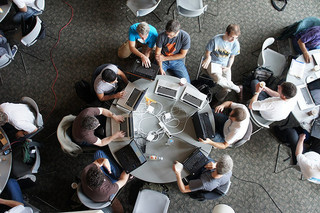
\includegraphics[width=0.6\textwidth]{images/common-property.jpg}\\
Sdílené intelektuální spoluvlastnictví
}

\only<3->{
    \begin{itemize}
        \item publikuj (aby ostatním \emph{studovat})
        \item ověření
        \item změnit a dále publikovat
    \end{itemize}
}

\note<1>{Protože je to otevřený systém
- systém, ve kterém ostatní sdílí svůj kód - svoje know-how - svoje
 intelektuální vlastnictví s ostatními.
 }
\note<2>{Ale koncept sdílení není přece vynalezen v 80 letech. Západní věda tak jak ji
chápeme je snad od dob antiky postavena na stejných principech:}

\note<3->{

\begin{itemize}
\item<3-5>publikuji výsledek způsobem, že je opakovatelný
\item<4-5>očekávám, že někdo jiný mou práci zopakuje přezkouší její platnost
\item<5-5>případně navrhne některé změny, a výsledek opět publikuje.
\end{itemize}
}
\note<6>{
Vědecká komunita díky sdílení informací posouvá hranice našeho
poznání dále, stejně jako komunita vývojářská posouvá hranice software.
}
\end{center}\end{frame}

\begin{frame}\begin{center}

\includegraphics[width=0.6\textwidth]<1>{images/wikipedia.jpg}
\includegraphics[width=0.6\textwidth]<2>{images/osm-logo.png}
\only<3>{
    \begin{itemize}
        \item prohlížet, studovat
        \item sdílet
        \item měnit a změny sdílet
    \end{itemize}
}


\note<1>{Open source software není jediný příklad pro fungující intelektuální
spoluvlastnictví. Nikdo snad nepochybuje, že wikipedia je spolehlivý informační
zdroj a přitom na její obsah nemá nikdo monopol, neexistuje globální autorita,
která by strážila věcný obsah Wikipedie.}

\note<2>{OpenStreetMap je podle mě další
úspěšný projekt. Jako geoprostoroví profesionálové můžete zpochybňovat polohovou
přesnost dat, jejich faktickou správnost nebo aktuálnost, ale nemůžete
zpochybnit, že globálně vzato je to ucelený dataset který nemá v prorietárním
světe obdoby.}

\note<3>{
    Všechny tyto příklady mají díky svým licencím společné tři základní vlastnosti,
které vyzývají další a další uživatele aby se přidali: vidět obsah, sdílet obsah
a provádět změny v obsahu a sdílet tyto změny dál.
}

\end{center}\end{frame}

\begin{frame}\begin{center}
\includegraphics[width=0.5\textwidth]<2>{images/Grasslogo_vector_big.png}
\includegraphics[width=0.5\textwidth]<3>{images/QGis_Logo.png}
\includegraphics[width=0.5\textwidth]<4>{images/Gdal-logo.png}
\includegraphics[width=0.5\textwidth]<5>{images/logo-PostGIS.png}
\includegraphics[width=0.9\textwidth]<6>{images/cuzk-portal.png}
\includegraphics[width=0.5\textwidth]<7>{images/mapserver-logo.png}

\note<1>{Open Source a geoinformační technologie: co k tomu říct}
\note<2-7>{Všichni jste slyšeli o
    \begin{itemize}
        \item GRASS GIS \textbf{NEXT}
        \item mnozí mají na svých počítačích QGIS \textbf{NEXT}
        \item většina používá knihovnu GDAL anižby o tom věděla, jsouc používána
            mimo jiné v ESRI ArcGIS \textbf{NEXT}
        \item nebo asi tušíte, že místo prorietárních databázových systémů lze
            použít PostgreSQL s prostorovou nadstavbou PostGIS. \textbf{NEXT}
        \item Možná jste si všimli, že nejeden český velký geoportál
používá pro zobraní mapové části knihovnu OpenLayers \textbf{NEXT}
        \item a už jste slyšeli, že MapServer je skutečně mapový server.
    \end{itemize}
}
\end{center}\end{frame}

\begin{frame}\begin{center}
\includegraphics[width=0.9\textwidth]<1>{images/Osgeolive_wordle.png}
\note<1>{Je jen málo oblastí geoinformatiky, které by nebyly pokryty kvalitním open
    source software - i když připouštím, že jsou. Stále vznikají nové programy pro
    další oblasti, staré ozkoušené projekty jsou ale stále zde, stabilní, s
    rozšířenou vývojářskou a uživatelskou komunitou, stále dostávají nové funkce, ty
    staré jsou oprašovány a udržovány.
}
\end{center}\end{frame}

\begin{frame}\begin{center}

\only<1>{
    \begin{exampleblock}{}
        \large Po dlouhé době jsem si na konferenci nemohl vybrat na kterou
        sekci půjdu, protože jsem chtěl být alespoň na třech najednou.
        \vskip5mm
        \vfill{\small --- Karel Charvát, FOSS4G 2011, Denver}
    \end{exampleblock}
}

\includegraphics[width=1\textwidth]<2>{images/vienna_code_sprint_pano_small.jpg}

\note<1>{
Pokud jste ještě nebyli na žádné konferenci zabývající se obecně geo* open source
software, doporučuji vám navštívit některou z konferencí FOSS4G, ať už letos ve
Spojených státech globální, nebo její evropskou odnož v Brémách.
}
\note<2>{Máte také
možnost nahlídnout přímo do  vývojářské kuchyně na některém z code sprints,
naposledy ve Vídni, další možnost budete mít v italském Bozlanu. 
}

\end{center}\end{frame}

\begin{frame}\begin{center}

\includegraphics[width=0.4\textwidth]{images/short_answers_headscratch.png}

\note<1>{
    Z toho všeho co říkám si možná říkáte: proč to tedy nidko nepoužívá, když je to
    tak skvělý produkt? Proč není open source software dávno rozšířenější, než jak
    to vypadá?

    Důvody pro tento stav - a je jedno jestli je to objektivní fakt nebo subjektivní
    pocit - jsou samozřejmě mnohé a jak už to bývá, mají povahu vnitřní i vnější.
}
\note<2>{Jako jeden z prvních důvodů (bez nároku na prvenství z hlediska významosti)
uvedu to, že člověk používá to, co zná. Věřím, že obsahem výuky na
školách ve všech oborech a stupních by měly být především obecně platné
principy, až od nich odvozené konkrétní situace.}
\end{center}\end{frame}

\begin{frame}\begin{center}
\includegraphics[width=0.4\textwidth]<1>{images/archim.jpg}
\includegraphics[width=0.7\textwidth]<2>{images/ponorka.png}
\includegraphics[width=0.7\textwidth]<3>{images/pocitace.jpg}
\note<1>{Učíme obecně Archimedův zákon}
\note<2>{a teprve následně několik jeho praktických aplikací, jako že ve vodě je slon
lehčí nebo spolu s inženýry španělského námořnictva, že ponorka, má-li se vynořit,
musí mít především v součtu menší objemovou hustotu, než voda.}
\note<3>{Proč se ale tento
princip uplatňuje při výuce software jen velice zřídka? Proč výuka počítačí
obecně a GIS konkrétně se téměř bez výjimky provádí na konkrétním jednom
software?}
\end{center}\end{frame}

\begin{frame}\begin{center}
\includegraphics[width=0.6\textwidth]<1>{images/empty-office.jpg}
\note<1>{Dalším důvodem je neexistejce jednohého telefonního čísla - chybí marketingové
oddělení open source GIS, není tu někdo, kdo by zákazníkům vysvětlil proč je
konkrétní produkt ten nejlepší (v absolutním i relativním významu). U open source
software se předpokládá, že jste dospělí, že jste nebo se chcete stát experty a
proto na to, co je pro váš případ to nejlepší si přijdete sami. Open source je
náročný na lidské zdroje, pokud nemáte u sebe někoho dalšího, jste v tom tak
trochu sami, "jenom" s podporou komunity. To může hodně lidí odradit, ale
bylo mnohokrát  dokázáno, že podpora komunity funguje, první odpověď v mailing
listech bývá u větších projektů v řádu minut.}

\end{center}\end{frame}

\begin{frame}\begin{center}
\includegraphics[width=0.6\textwidth]<1>{images/stamp.jpg}
\note<1>{Dalším důvodem je nejednotný systém návazného vzdělávání. Existují spíše
jednotlivci, nebízející školení. Školení jsou ale nejednotná, různá obsahem i
kvalitou. V zahraniční vznikají certifikační projekty, k nám zatím nedorazily.
}

\note<2>{
Důvodů, proč open source software není úspěšnější - myšleno absolutně - je ještě
celá další řada. Některé z nich a některé z již zmíněných se bude snažit zaplnit
na naší geo- scéně projekt GISMentors.
}

\end{center}\end{frame}

\begin{frame}\begin{center}
\note{
Projekt GISMentors je společný projekt několika jednotlivců, kteří se rozhodli
spojit své síly a nabídnout pod společnou hlavičkou kvalitní školení pro
co nejširší oblast open source GIS. Školení budou obsahovat všechno to, na co
jsou účastníci podobných akcí zvyklí, ale ještě i něco navíc -- účastníci si
odnesou s sebou domů i software, na kterém školení probíhalo spolu s daty, která
byla použita. Doufáme, že se nám tak podaří snížit jednu z bariér pro větší
rozšíření open source software pro geoprostorové informace.
}
\end{center}\end{frame}

\begin{frame}\begin{center}
\includegraphics[width=0.6\textwidth]<1>{images/marketing.jpg}
\note{
Takže věříme, že budete-li mít v budoucnu problém s open source software pro GIS
nebo budete-li si chtít doplnit vzdělání, budete mít kde.
}
\end{center}\end{frame}

%\begin{frame}\begin{center}
%\end{center}\end{frame}

\section*{Závěr}
\begin{frame}
    Dotazy?
\note{Děkuji Vám za pozornost, kterou jste mi věnovali a jsem připraven
odpovědět na vaše dotazy, máte-li nějaké}
\end{frame}


\end{document}
